
    \subsection*{Example of Activation Functions}
    
        So, let's look at some possible \textbf{activation} functions:
        
        \begin{itemize}
            \item \vocab{Step} function $\text{step}(z)$:
            
                \begin{equation}
                    \text{step}(z) 
                    =
                    \begin{cases}
                      1 & \text{if $z \geq 0$}\\
                      0 & \text{if $z < 0$}
                    \end{cases}
                \end{equation}
                
                \begin{figure}[H]
                    \centering
                    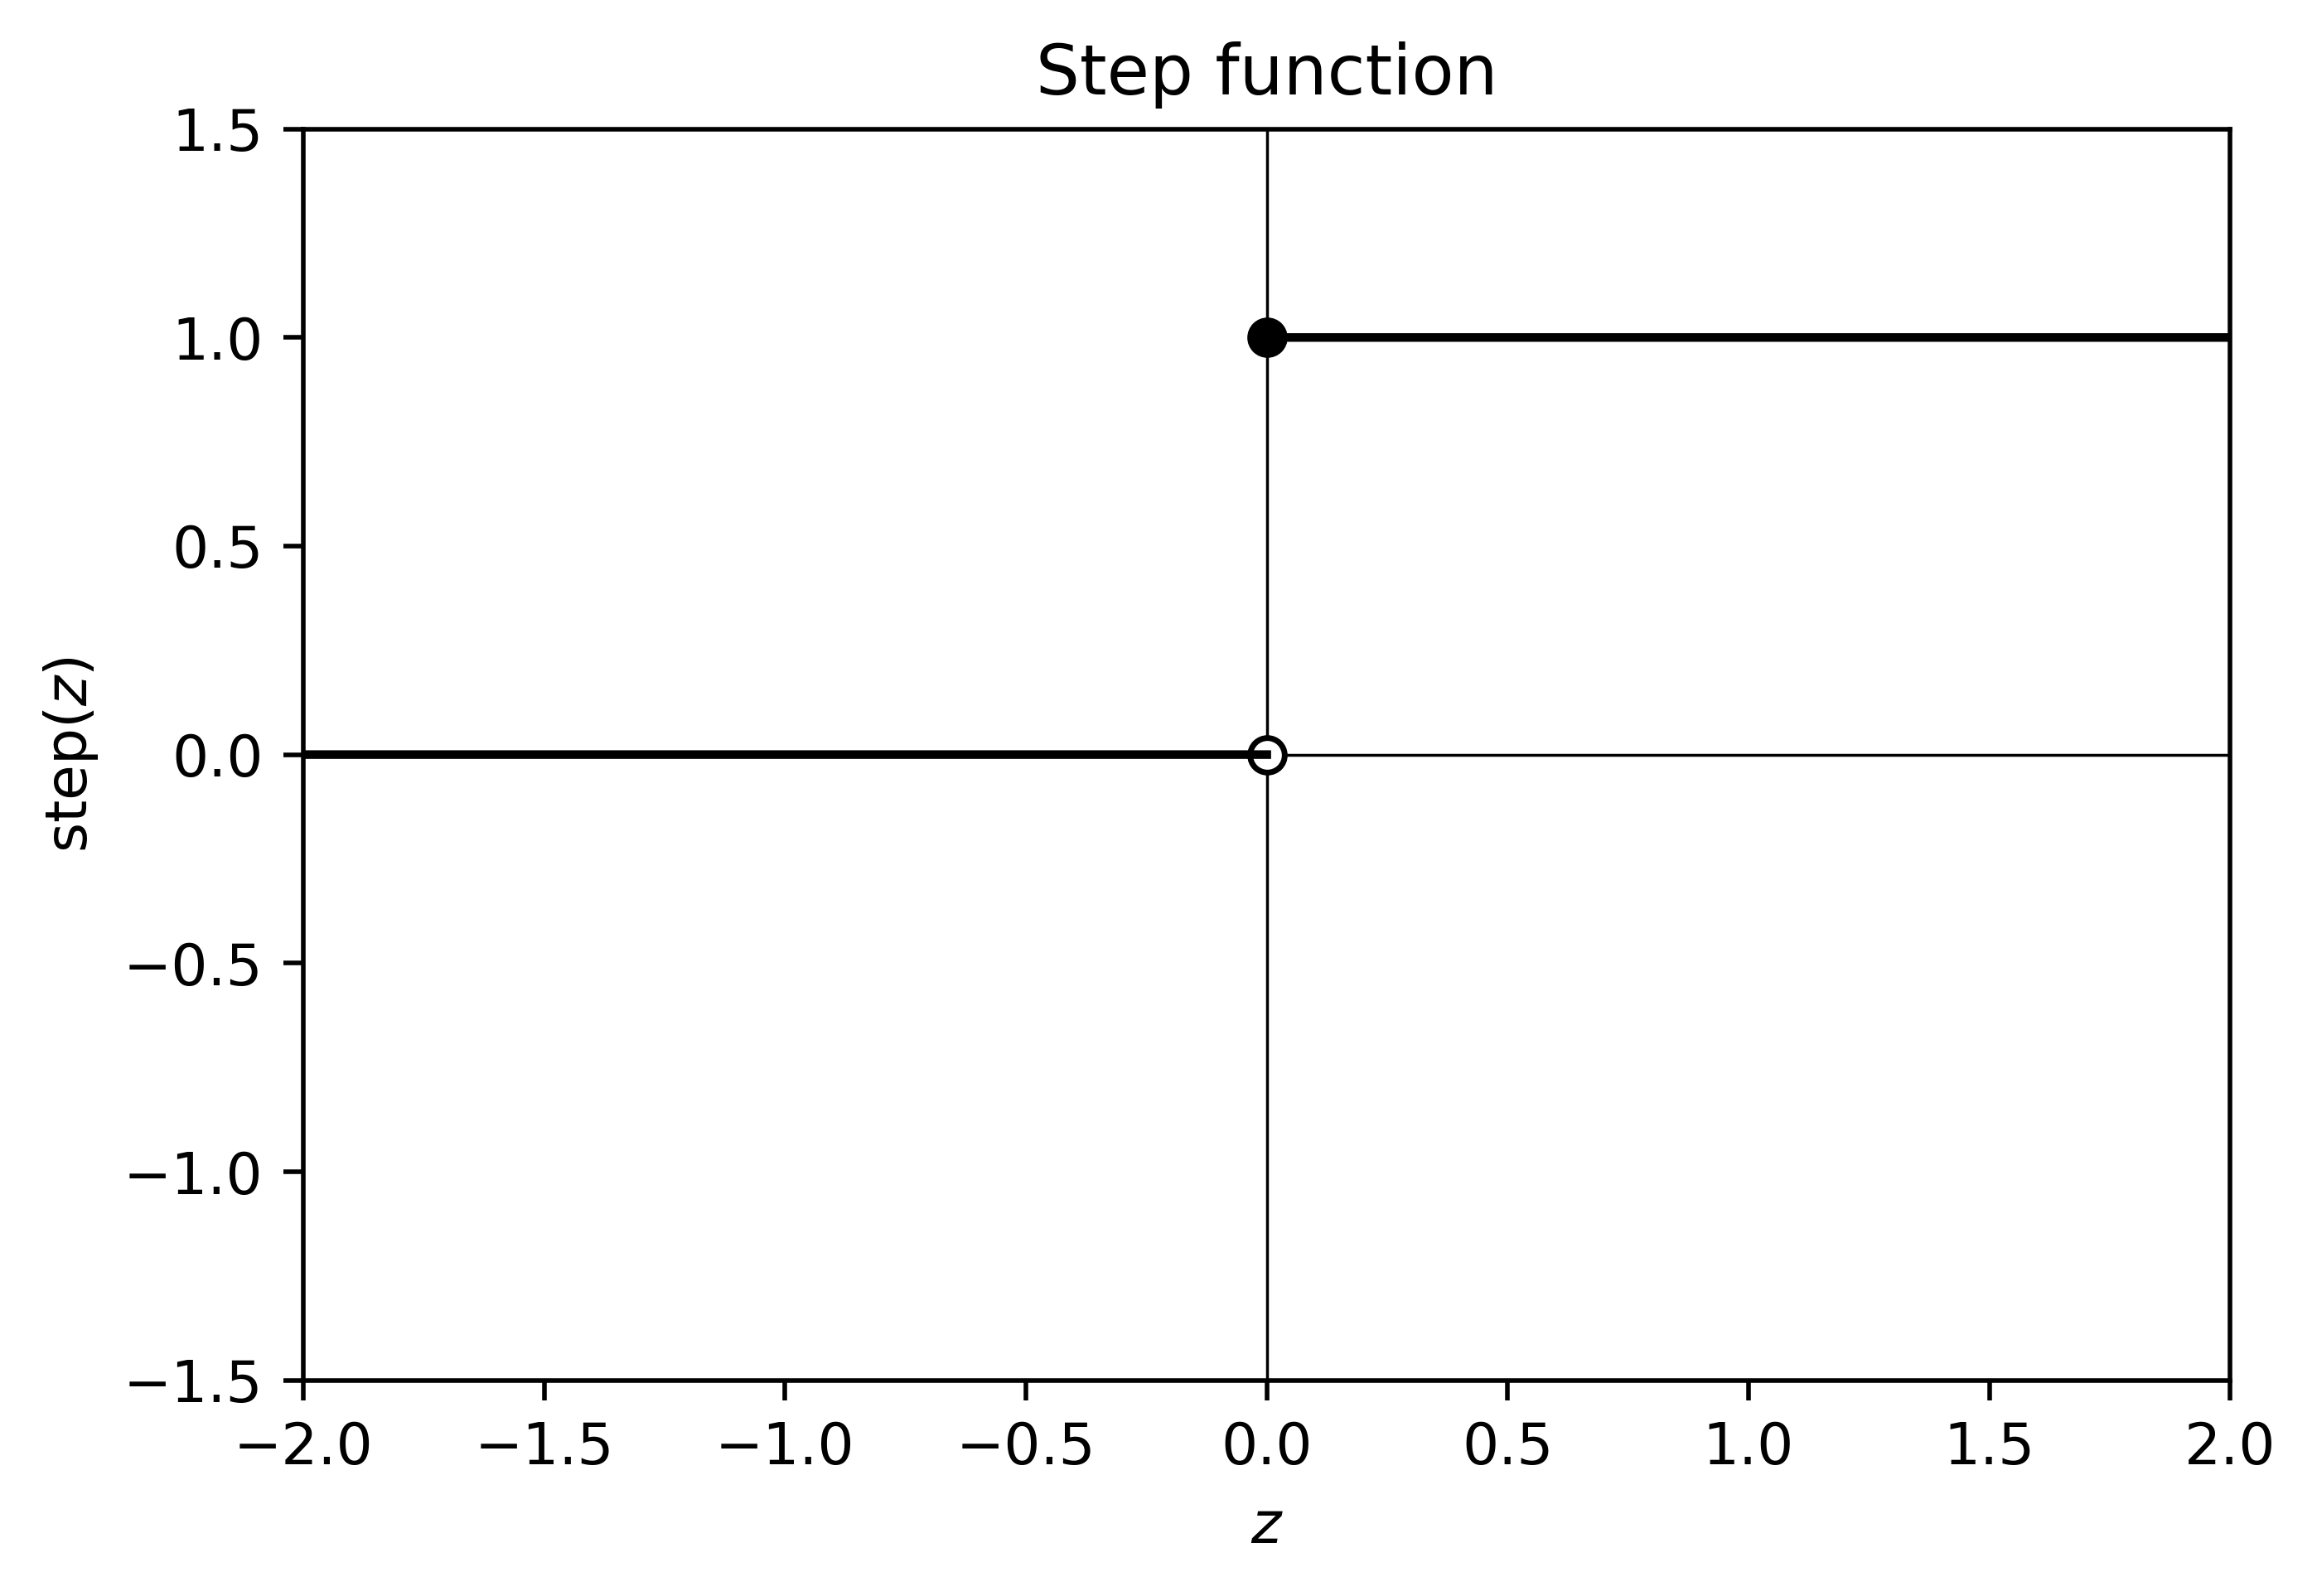
\includegraphics[width=60mm,scale=0.4]{images/nn_images/step_fn.png}
                \end{figure}
                
                \begin{itemize}
                    \item This function is basically a \textbf{sign} function, but uses $\{0, 1\}$ instead of $\{-1, +1\}$.
                    
                    \item Step functions were a common early choice, but because they have a \textbf{zero} gradient, we can't use \textbf{gradient descent}, and so we basically \textbf{never} use them.
                        \note{Same reason we replaced the sign function with sigmoid.}
                \end{itemize}
            
            
            \item \vocab{Rectified Linear Unit} ReLU$(z)$:
            
                \begin{equation}
                    \text{ReLU}(z) 
                    =
                    \max(0,z)
                    =
                    \begin{cases}
                      z & \text{if $z \geq 0$}\\
                      0 & \text{if $z < 0$}
                    \end{cases}
                \end{equation}
                
                \begin{figure}[H]
                    \centering
                    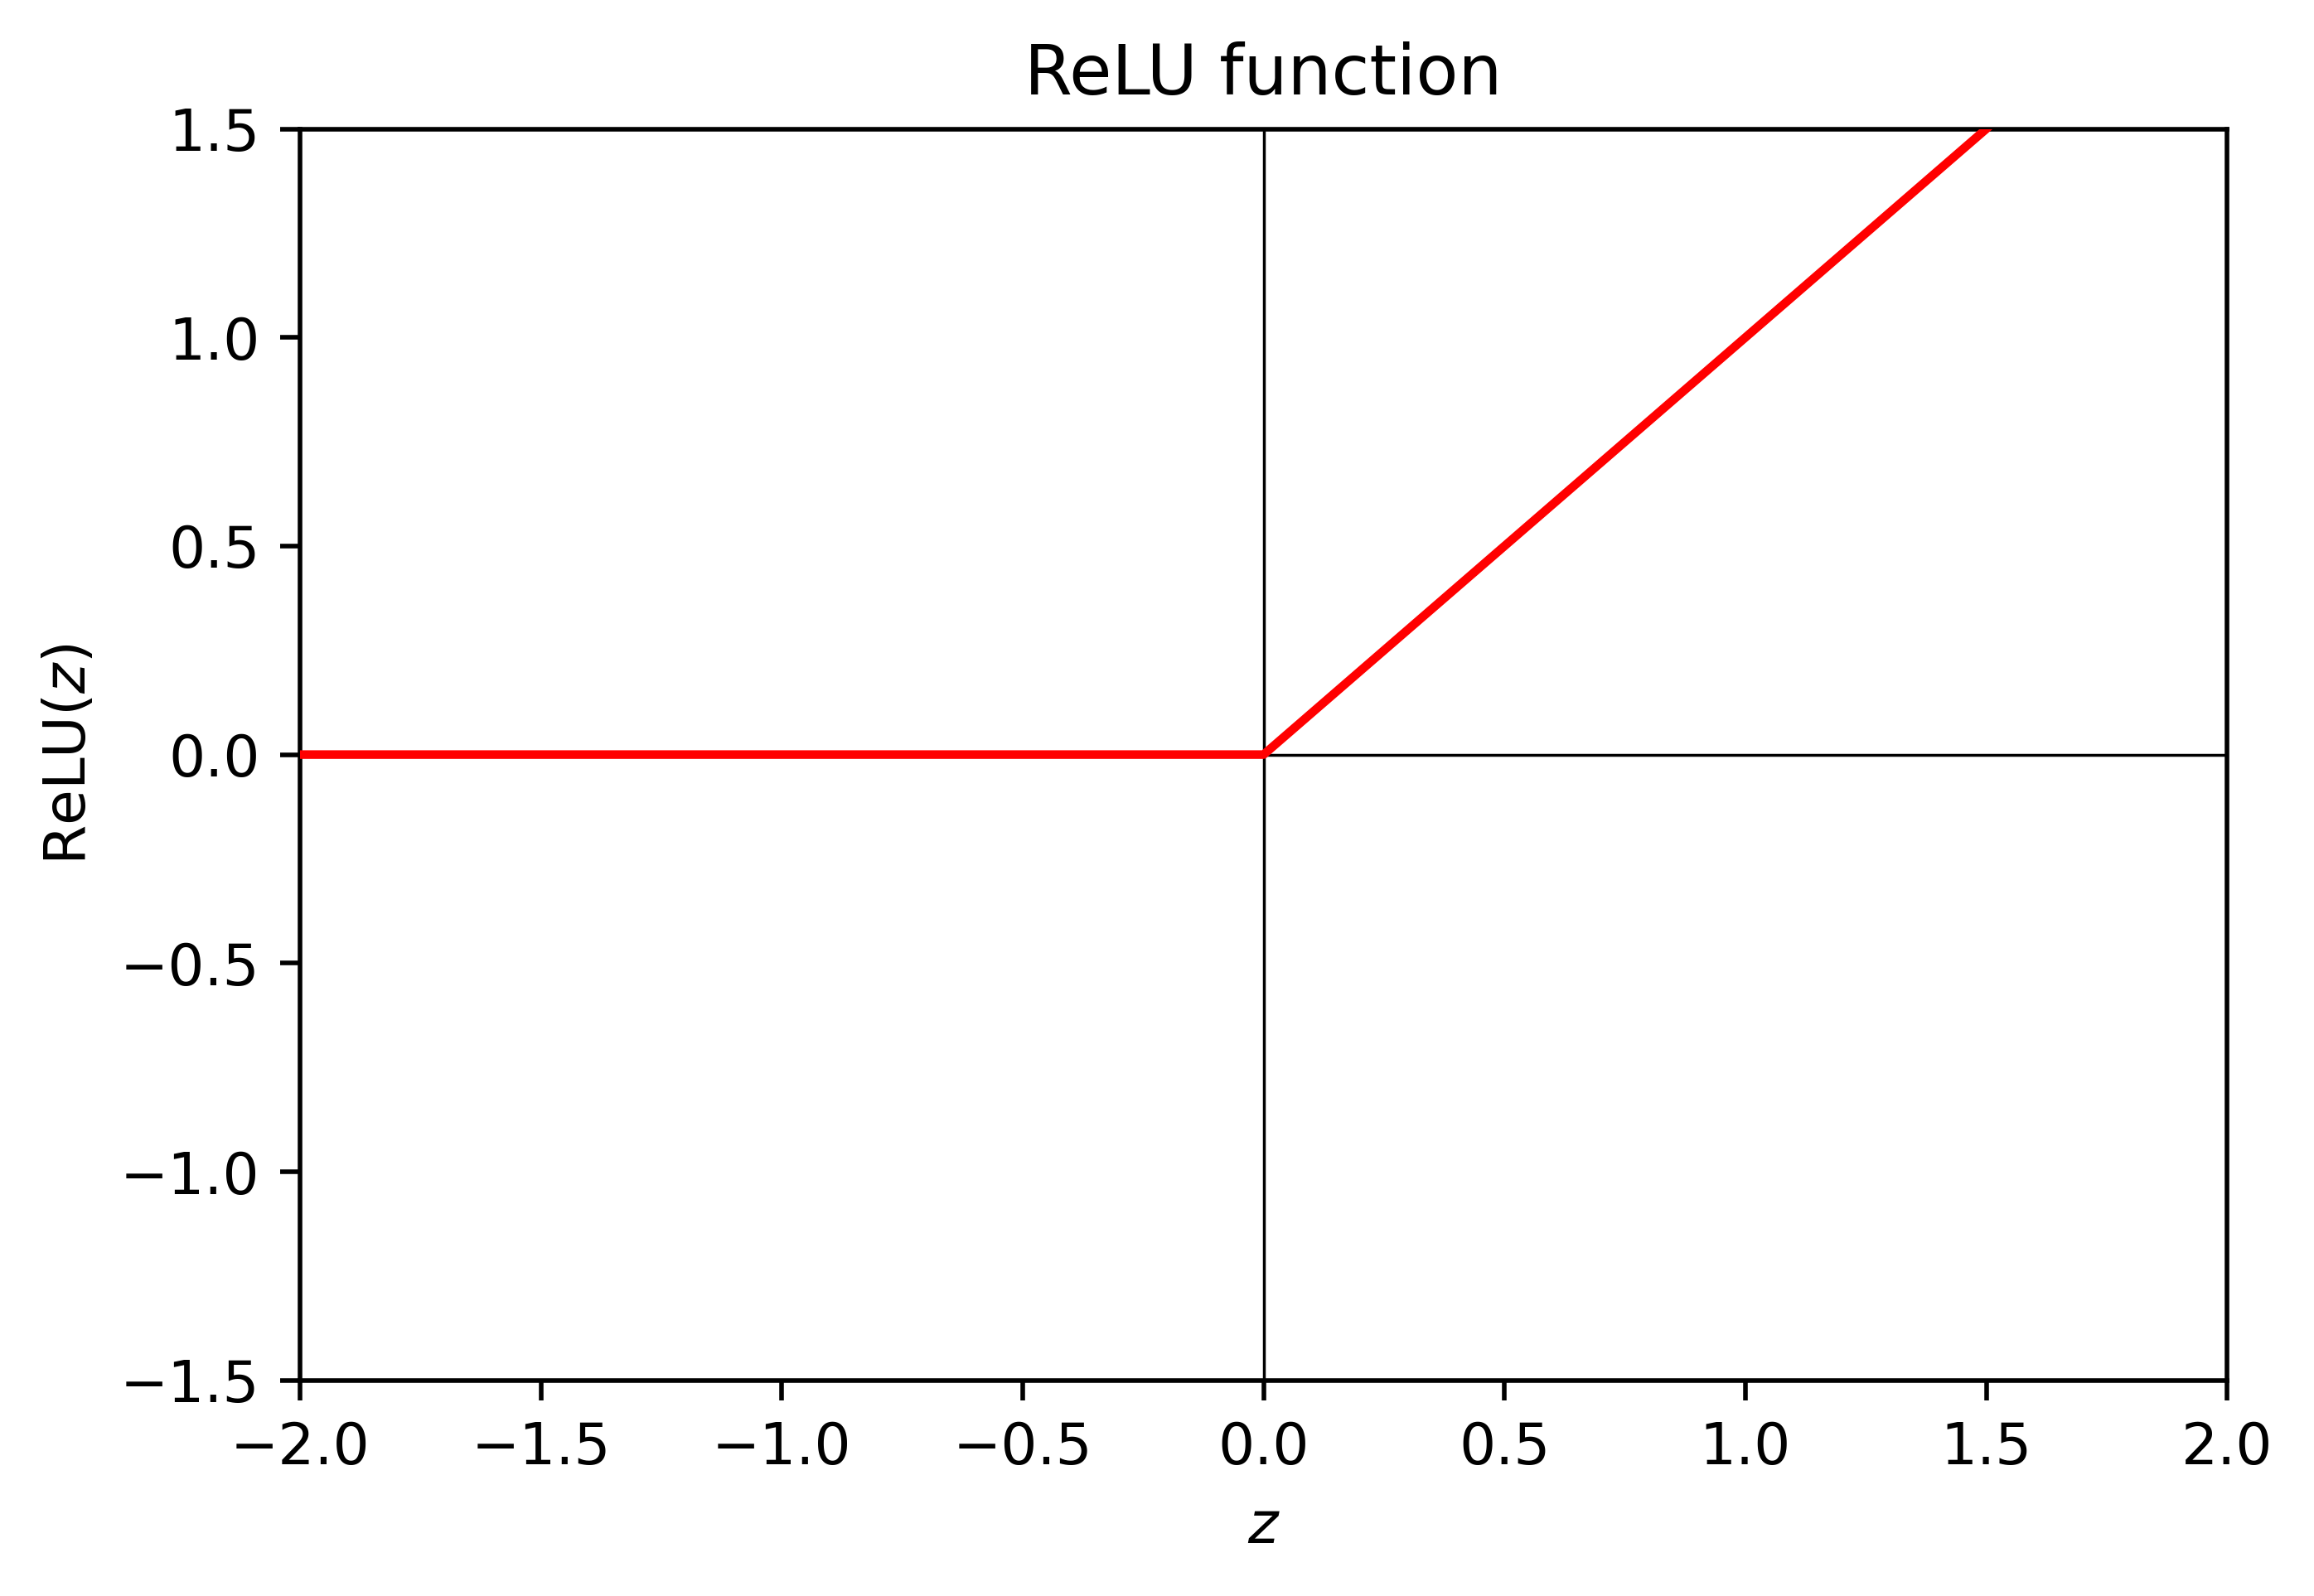
\includegraphics[width=60mm,scale=0.4]{images/nn_images/relu_fn.png}
                \end{figure}
                
                \begin{itemize}
                    \item This is a very \textbf{common} choice for activation function, even though the derivative is undefined at 0.
                    
                    \item We specifically use it for internal ("\textbf{hidden}") layers: layers that are neither the \textbf{first} nor \textbf{last} layer.
                        \note{They're "hidden" because they aren't visible to the input or output.}
                \end{itemize}
            
            
            \item \vocab{Sigmoid} function $\sigma(z)$:
            
                \begin{equation}
                    \sigma(z) = \frac{1}{1+e^{-z}}
                \end{equation}
                
                \begin{figure}[H]
                    \centering
                    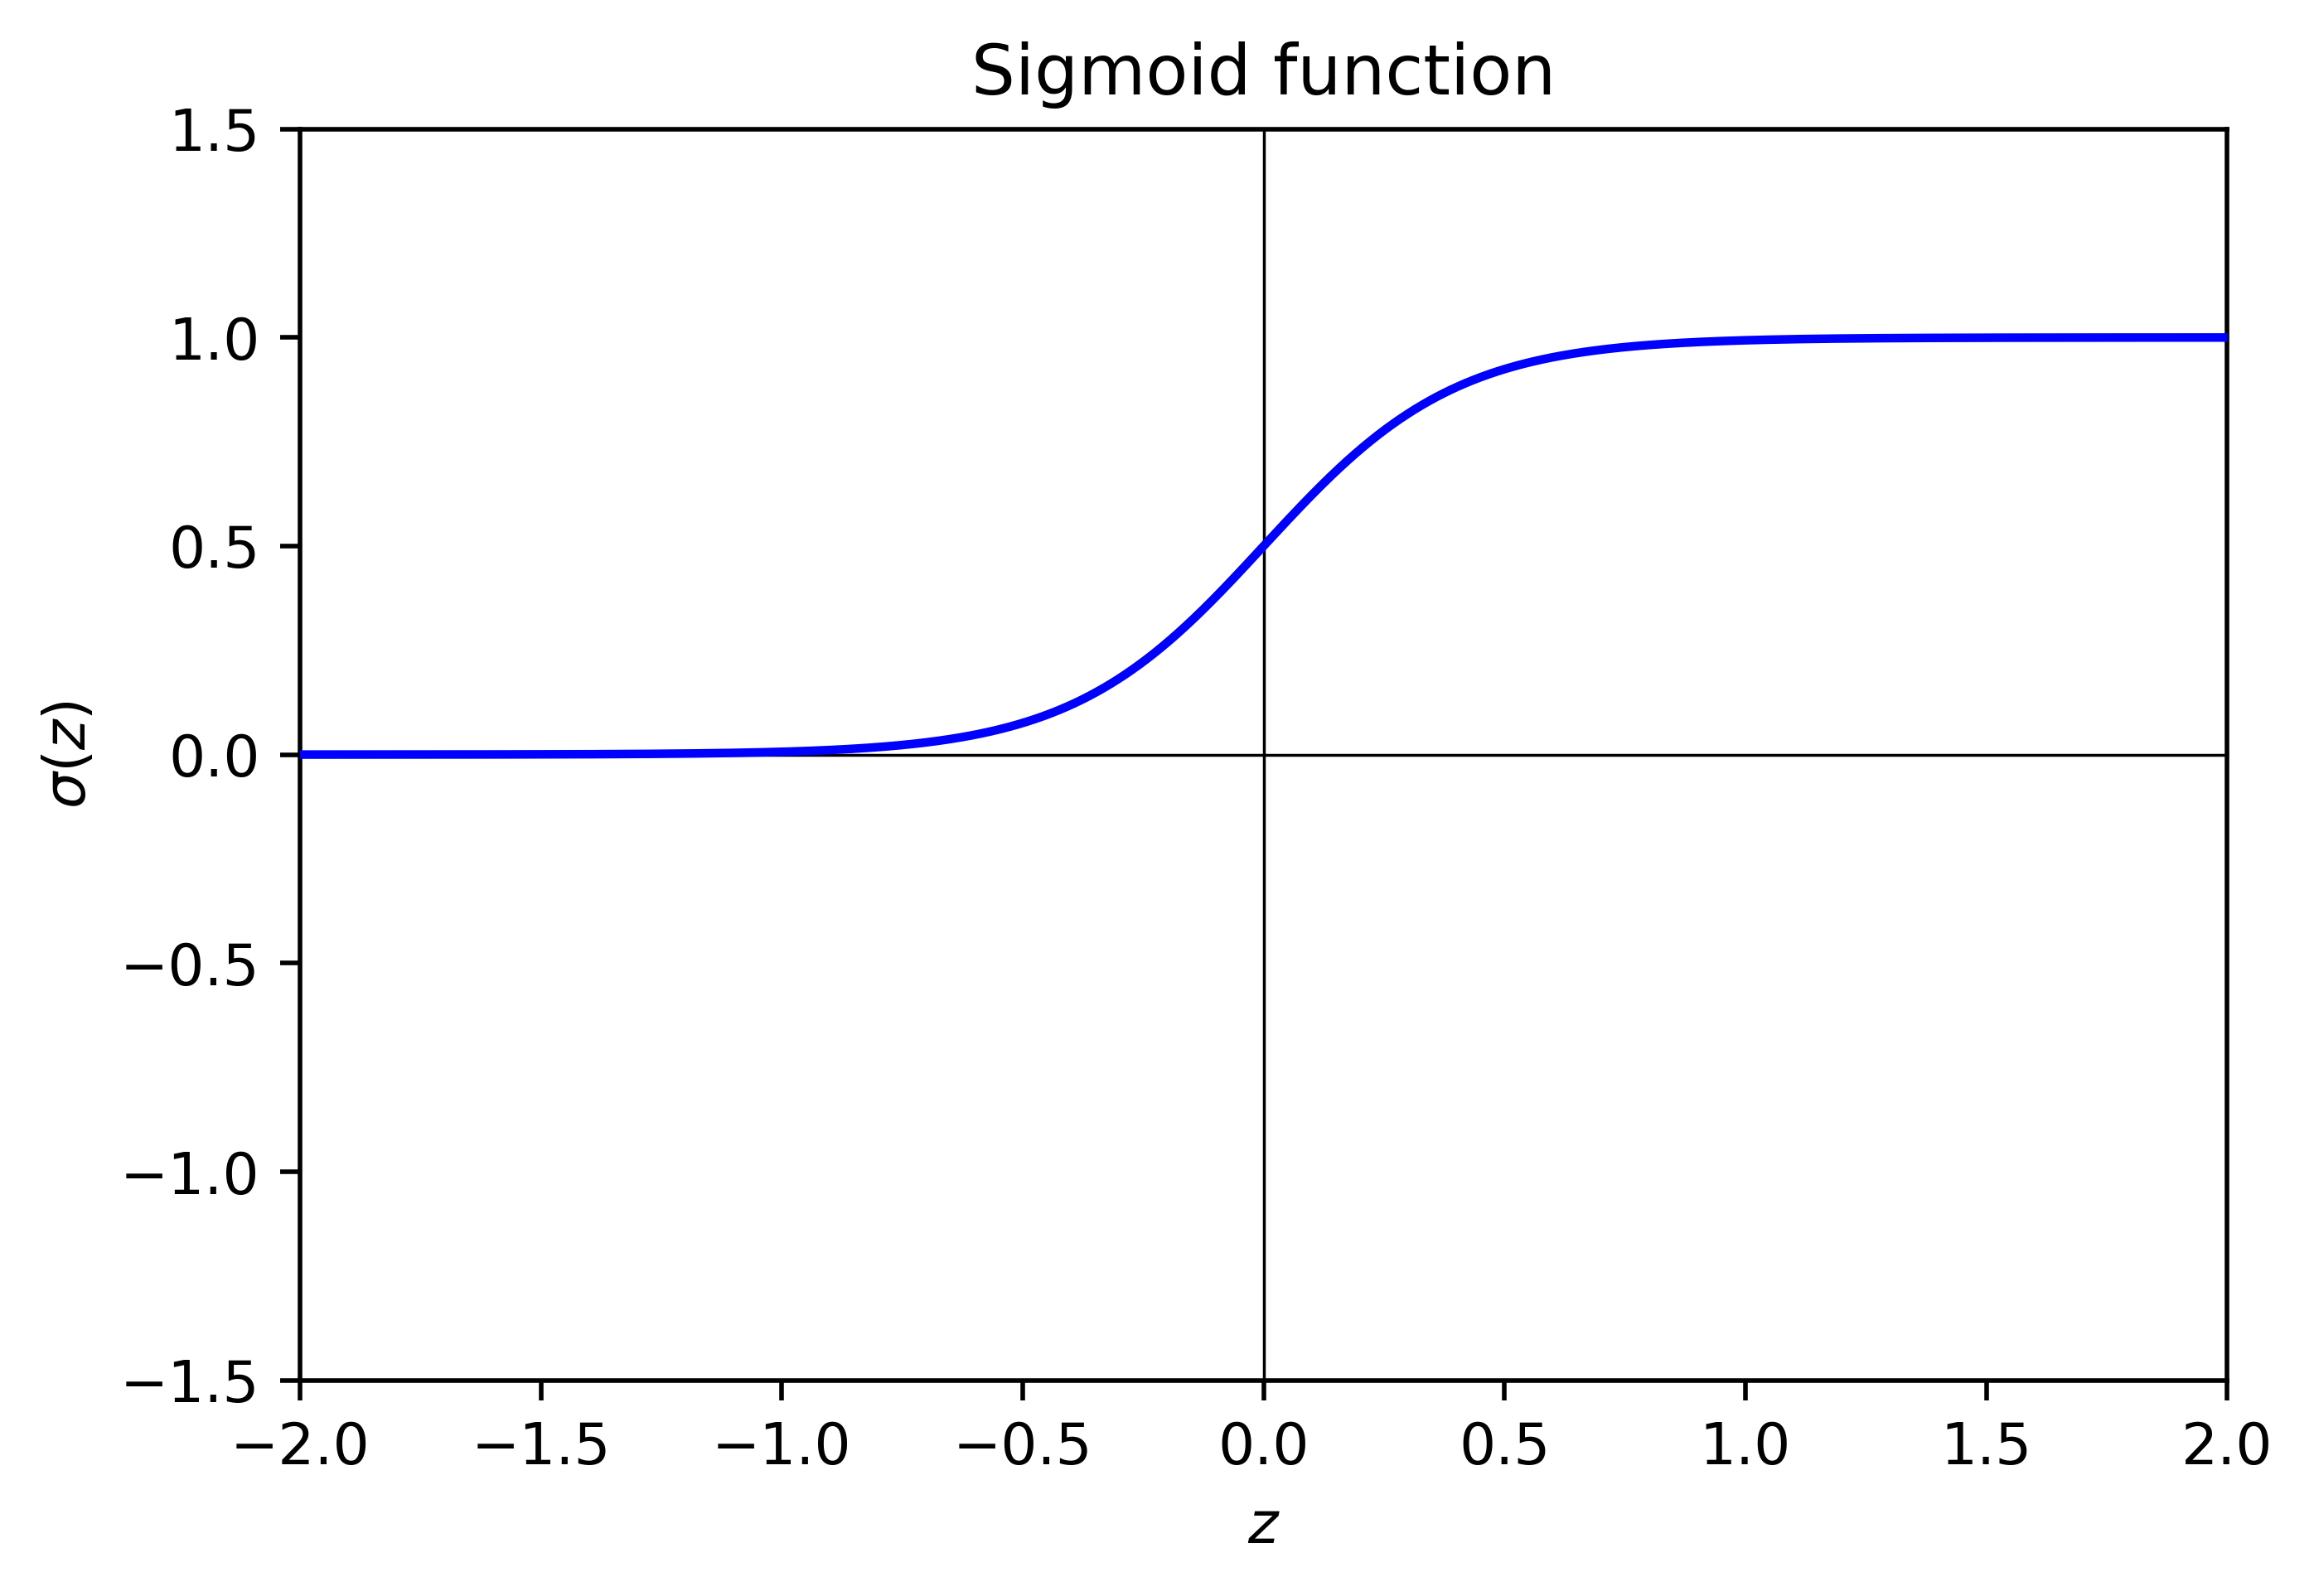
\includegraphics[width=60mm,scale=0.4]{images/nn_images/sigmoid_fn.png}
                \end{figure}
            
                \begin{itemize}
                    \item This is the \textbf{activation} function for our \textbf{LLC} neuron from before.
                    
                    \item Just like it was then, it's useful for the \textbf{output neuron} in \textbf{binary classification}.
                    
                    \item Can be interpreted as the \textbf{probability} of a positive ($+1$) binary classification.
                \end{itemize}
                
            \item \vocab{Hyperbolic Tangent} $\tanh(z)$:    
                
                \begin{equation}
                    \tanh(z) = \frac{e^z - e^{-z}}{e^z + e^{-z}}
                \end{equation}
                
                \begin{figure}[H]
                    \centering
                    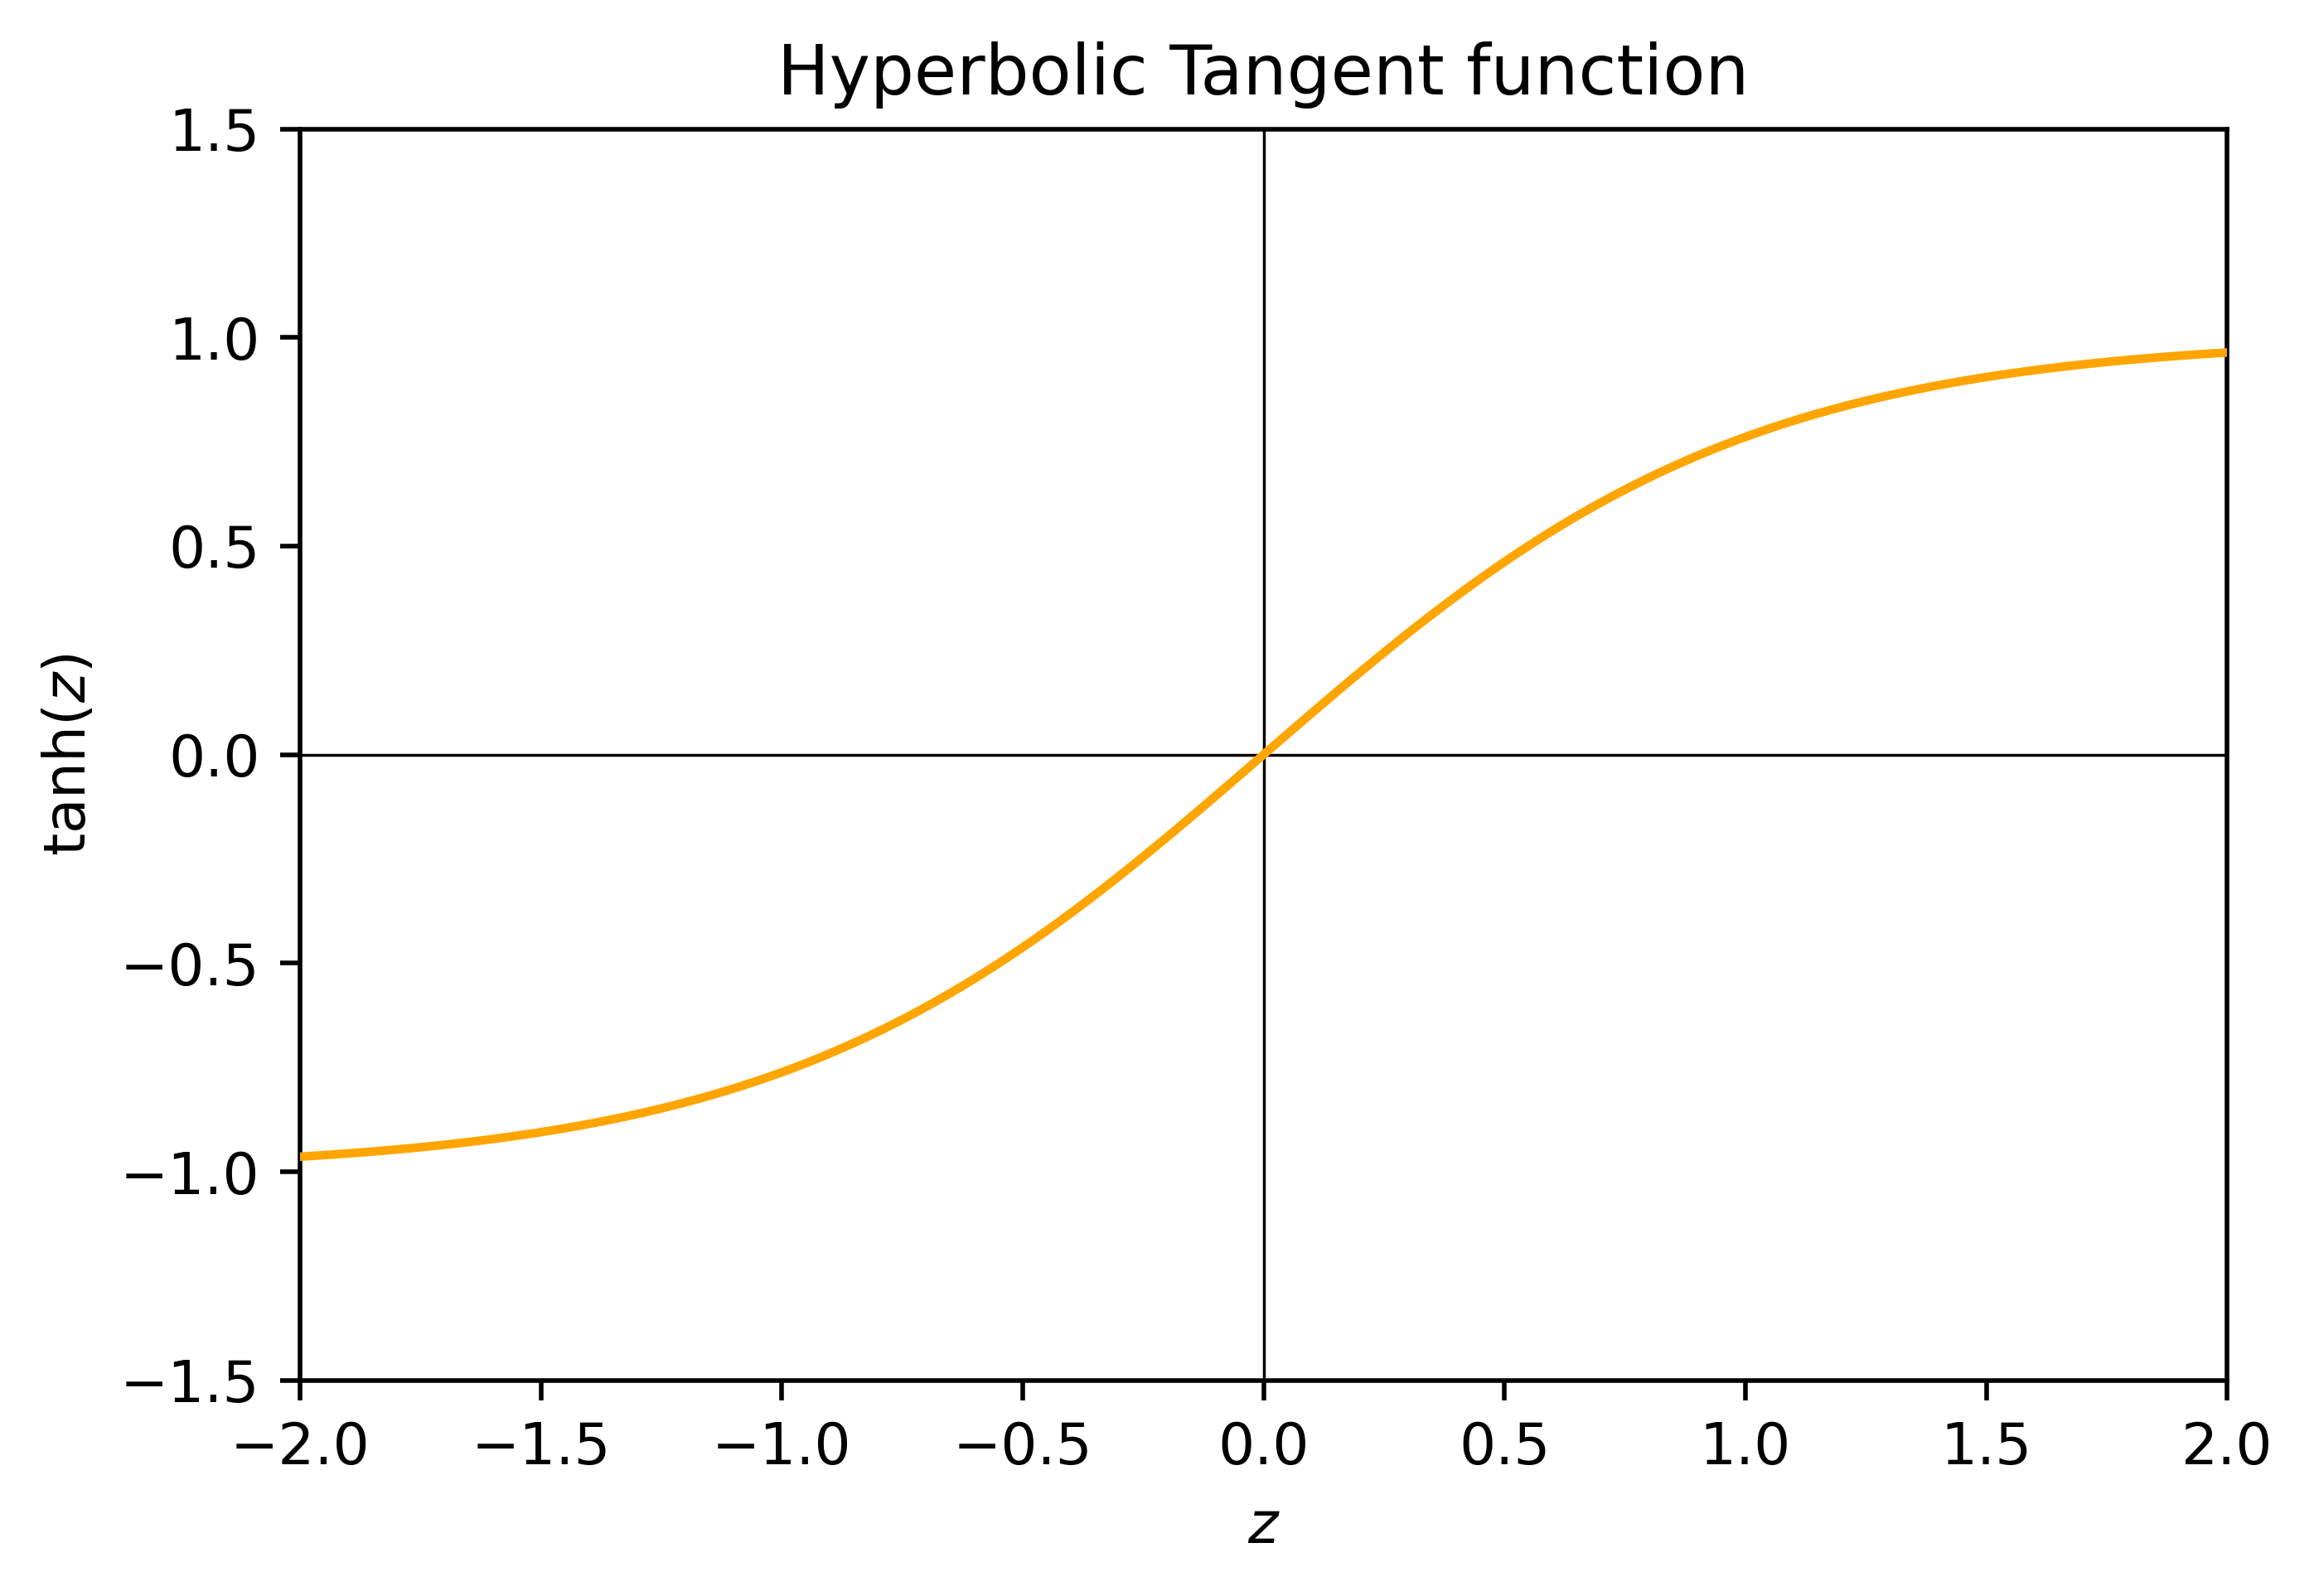
\includegraphics[width=60mm,scale=0.4]{images/nn_images/tanh_fn.png}
                \end{figure}
                
                \begin{itemize}
                    \item This is function looks similar to sigmoid over a different \textbf{range}.
                    
                    \item Unfortunately, it will not get much use in this class.
                \end{itemize}
                
            \item \vocab{Softmax} function softmax$(z)$:
                
                \begin{equation}
                    \text{softmax}(z) =
                    \begin{bmatrix}
                        \exp(z_1) / \sum_{i} \exp(z_i) \\
                        \vdots \\
                        \exp(z_n) / \sum_{i} \exp(z_i)
                    \end{bmatrix}
                \end{equation}
                
                \begin{itemize}
                    \item Behaves a like a \textbf{multi-class} version of \textbf{sigmoid}.
                    
                    \item Appropriately, we use it as the \textbf{output neuron} for \textbf{multi-class} classification.
                    
                    \item Can be interpreted as the \textbf{probability} of our $k$ possible classifications.
                \end{itemize}
        \end{itemize}
        
    \begin{concept}
        For the different \vocab{activation functions}:
        
        \begin{itemize}
            \item \blu{sign$(z)$} is \purp{rarely} used.
            
            \item \blu{ReLU$(z)$} is often used for "\purp{hidden}" layers.
            
            \item \blu{$\sigma(z)$} is often used as the \gren{output} for \purp{binary classification}.
            
            \item \blu{softmax$(z)$} is often used as the \gren{output} for \purp{multi-class classification}.
        \end{itemize}
        $\tanh(z)$ is useful, but not a focus of this class.
    \end{concept}
    
\pagebreak
%%%%%%%%%%%%%%%%%%%%%%%%%%%%%%%%%%%%%%%%%%%%%%%%%%%%%%%%%%%%%%%%%%%%%%%%%%%%%  
\section*{Loss functions and activation functions}

    As we can see above, your \textbf{activation} function depends on what kind of \textbf{problem} you're dealing with.
    
    The same is true for our \textbf{loss} function: we used \textbf{different} loss functions for classification and regression.
    
    Classification can be further broken up into \textbf{binary} versus \textbf{multiclass} classification.
    
    To summarize our findings, we'll \textbf{sort} this information:\\
    
    \begin{concept}
        Each of our \vocab{tasks} requires a different \purp{loss} and output \gren{activation} function.
        
        We emphasize that we specifically mean the \red{output} activation function: the activation function used in \gren{hidden layers} doesn't have to match the loss function.
        
        \begin{center}
            \begin{tabular}{c | c c | c c}
                task &  $f^L$ && Loss & \\
                
                \hline\hline
                
                \red{Regression}        & Linear    &  \red{$z$}  
                & Squared & \red{$(g-y)^2$} \\
                
                &&&&\\
                \hline
                
                \blu{Binary Class}      & Sigmoid   &  \blu{$\sigma(z)$ }
                & NLL & \blu{$y\log g + (1-y) \log (1-g)$}\\
                
                &&&&\\
                \hline
                
                \pur{Multi-Class}       & Softmax   &  \pur{softmax$(z)$} 
                & NLLM & \pur{$\sum_j y_jlog(g_j)$}\\
                
                &&&&\\
                
            \end{tabular}
        \end{center}
    \end{concept}
    